\chapter{Experimental methods}
\label{ch:methods}

\section{The Large Hadron Collider}

At the time of writing, the Large Hadron Collider~\cite{Bruning:2004ej} is the largest and most powerful particle accelerator in the world. Located underground at the border of France and Switzerland close to Geneva, it consists of two circular beamlines of roughly 27~km circumference, in which proton bunches are accelerated and collided. Superconducting magnets, cooled with liquid helium at around 4~K temperatures, generate magnetic fields of over 8~T to keep the protons on their circular orbit, and similarly superconducting electromagnetic radio-frequency cavities accelerate the protons to beam energies up to 7~TeV. When operating as designed, around 2800 proton bunches per beam containing $3\times10^{14}$ protons total are present in the beamline simultaneously, revolving with a frequency of about 11.245~kHz. From this, peak instantaneous luminosities of about \SI{20}{\kilo\hertz\per\micro\barn} can be reliably reached. Alternatively, the LHC can also collide heavy ions, such as lead or oxygen, instead of protons.

There are four large experiments making use of the colliding beams at the LHC, located at the four interaction points. The two larger of these are ATLAS~\cite{ATLAS:2008xda} and CMS~\cite{CMS:2008xjf}, both of which are general-purpose experiments intended to study all aspects of the Standard Model in proton-proton collisions. The work of thesis was performed as part of the CMS collaboration, and so the CMS experiment is described in \cref{sec:methods:cms} in more detail. The two smaller experiments, on the other hand, are specialized for certain tasks, namely the study of B physics and exotic hadrons for LHCb~\cite{LHCb:2008vvz} and the study of heavy-ion collisions for ALICE~\cite{ALICE:2008ngc}.

The data taken at the LHC so far can be divided into three Runs. Run~1 lasted from 2010--2012, during which the LHC operated at center-of-mass energies of 7 and 8~TeV, significantly below the original target values, and yielded a total integrated luminosity of about \SI{29}{\fbinv}. It is this data that led to the original discovery of the Higgs boson. Following this, after two years of pause, Run~2 resumed in 2015 with a center-of-mass energy of 13~TeV and lasting to 2018. Around \SI{140}{\fbinv} of data was collected during this time. This complete data set, save for the small contribution from 2015, is analyzed in \cref{ch:ah} of this thesis.

Finally, Run~3 of the LHC started in 2022 after another three years of pause, and is planned to last until 2026 at the time of writing. The center-of-mass energy was again increased slightly to 13.6~TeV, and in the years 2022--2024 around \SI{196}{\fbinv} have been recorded, already surpassing Run~2. In \cref{ch:ttxs} of this thesis, the very first data of Run~3, corresponding to \SI{1.21}{\fbinv} taken in July and August 2022 at CMS, are analyzed in the context of a \ttbar cross section measurement. 

In the future, it is planned to upgrade the LHC to be able to run at higher instantaneous luminosities as well as a further increased energy of 14~TeV~\cite{ZurbanoFernandez:2020cco}. The CMS detector will similarly be upgraded to replace aging components and deal with the increased pileup conditions~\cite{CMS:TDR-15-02,CMS:PRF-21-001}, and a total integrated luminosity of around \SI{3}{\abinv} is expected to be collected. In \cref{ch:alps}, among others, sensitivity projections for this luminosity are made for Axion-Like Particles decaying to \ttbar.

\section{The CMS experiment}
\label{sec:methods:cms}

The Compact Muon Solenoid experiment~\cite{CMS:2008xjf,CMS:PRF-21-001}, located at Interaction Point~5 of the LHC close to Cessy, France, is a general-purpose particle detector targeting a broad range of SM and BSM phenomena. Its main feature is a superconducting solenoid magnet creating a strong magnetic field of 3.8~T. CMS is a hermetic detector, covering almost the full solid angle in space, and is split into a \textit{barrel}, covering pseudorapidities of $\abseta \lesssim 1.5$, and two forward \textit{endcaps}, covering high \abseta values. It consists of several subdetectors, which are geared towards different particle types and properties.

\begin{figure}[!t]
    \centering
    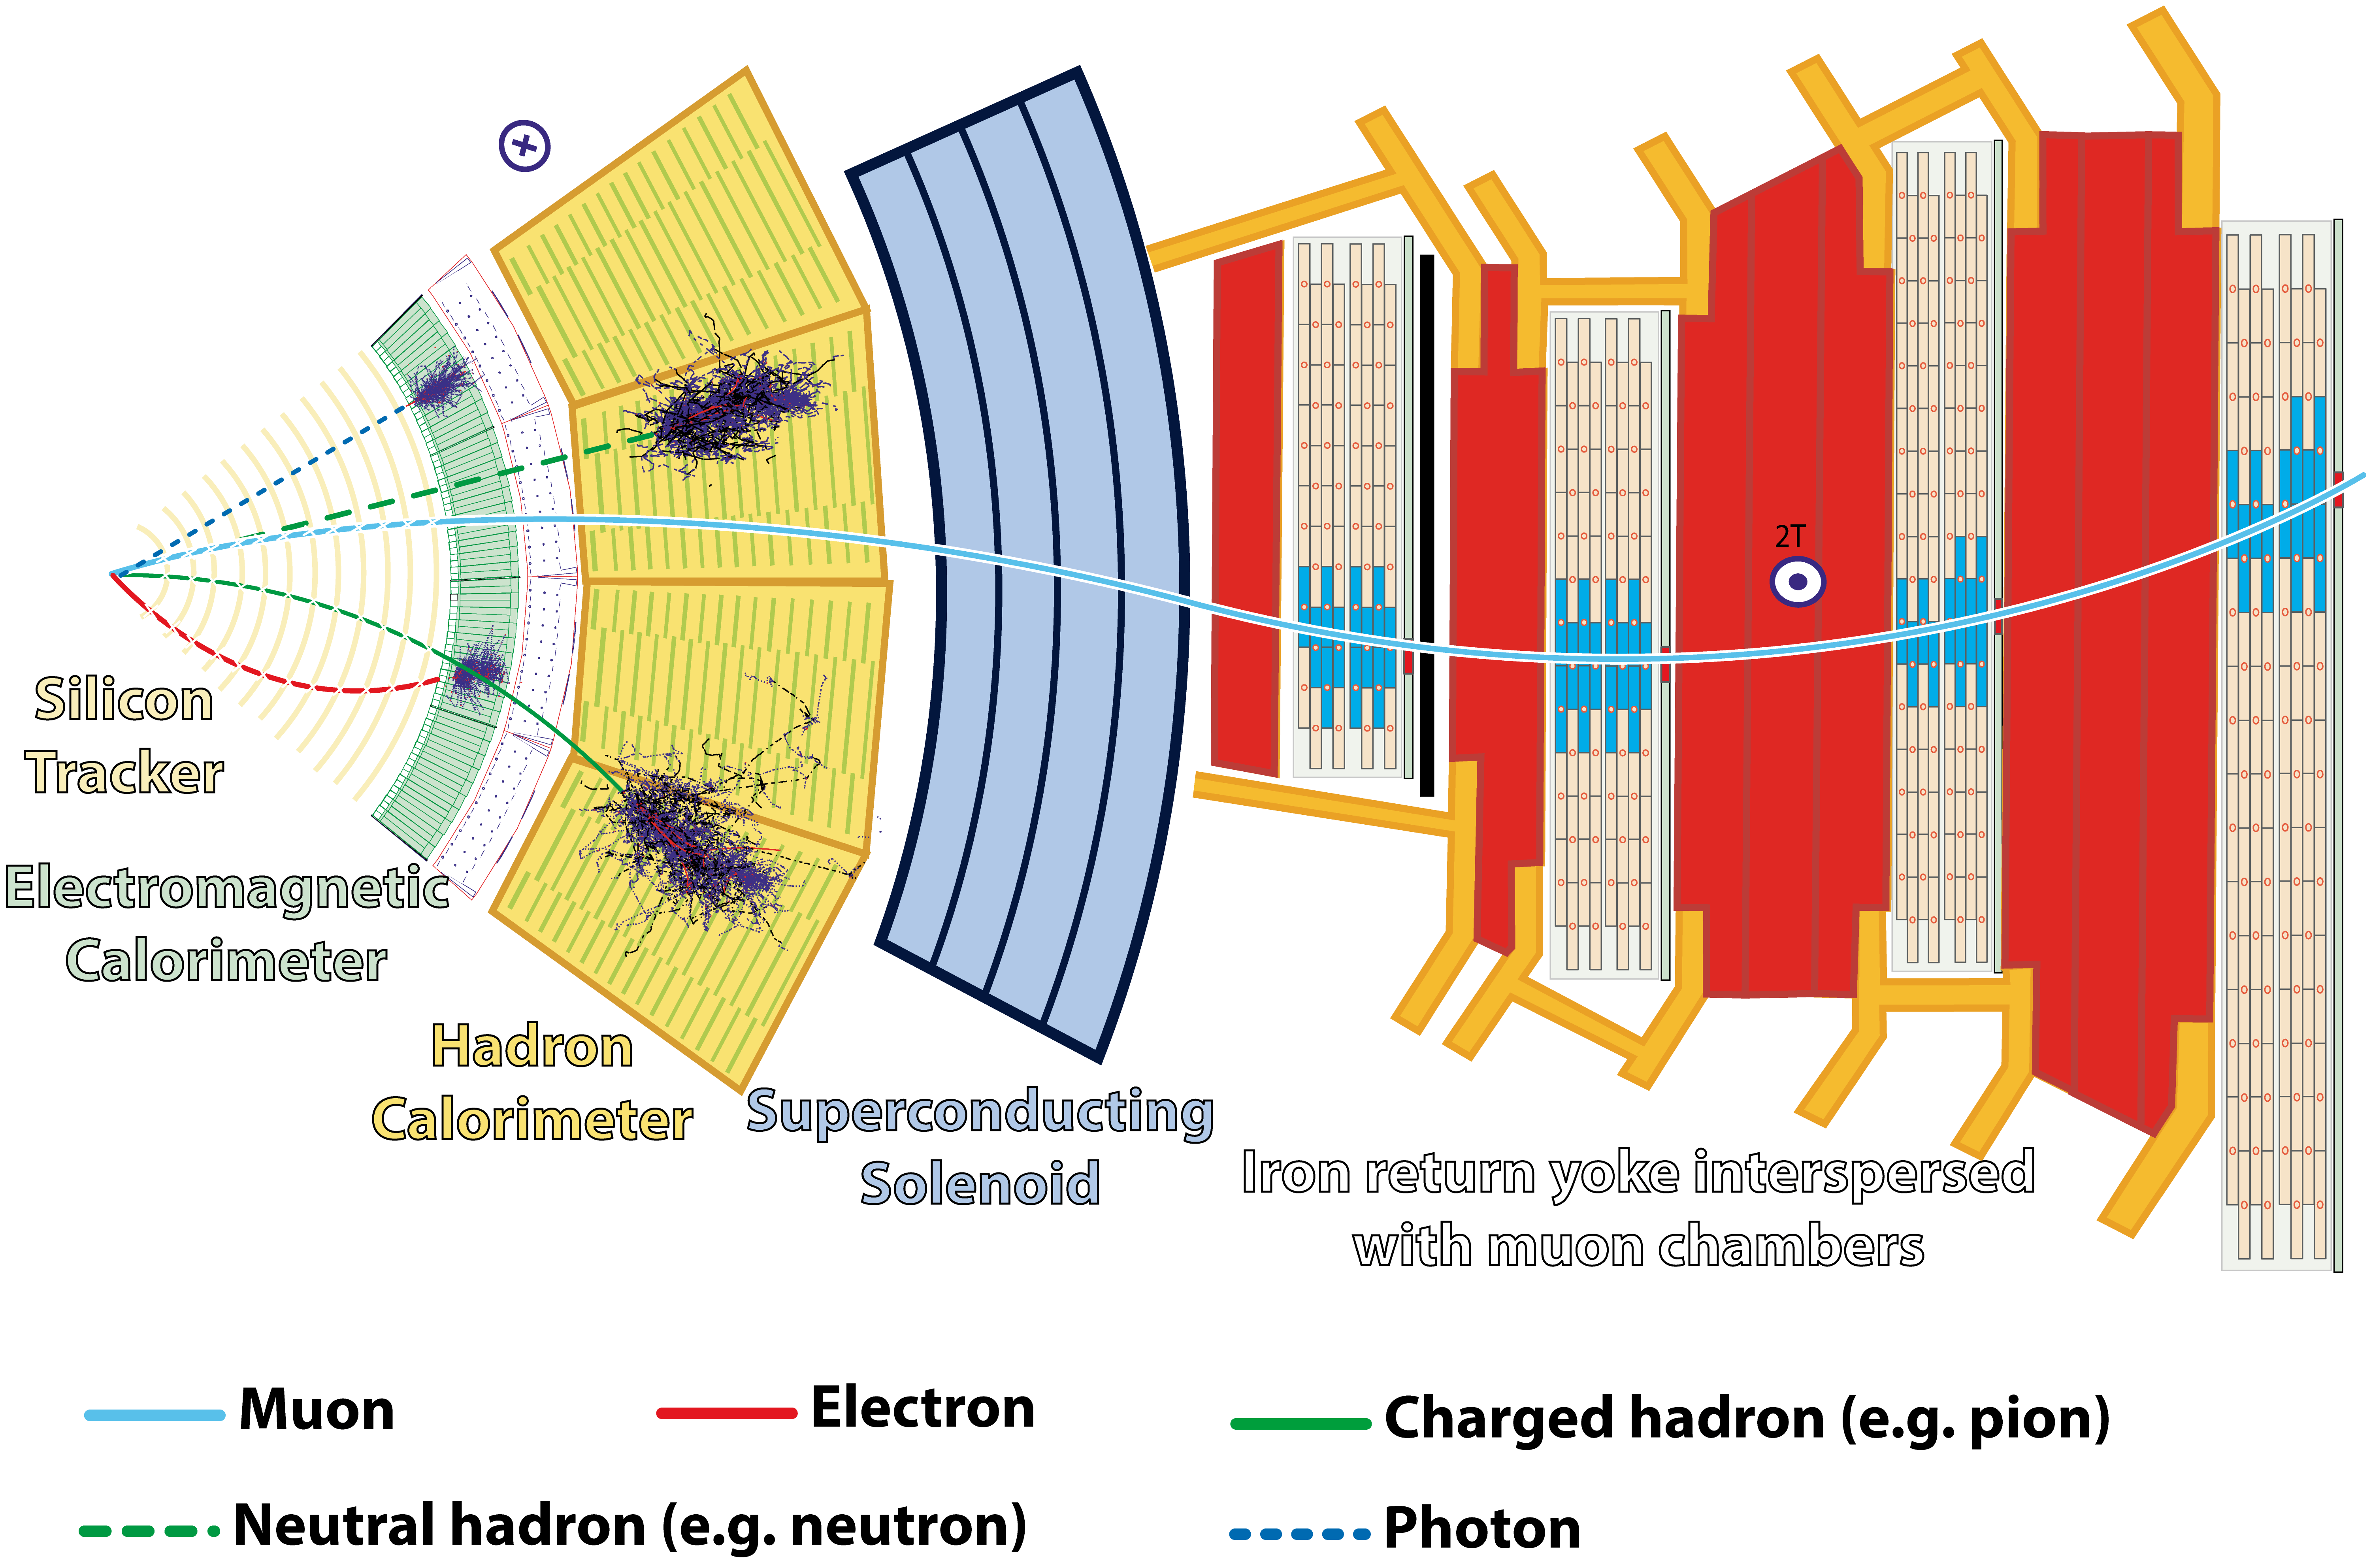
\includegraphics[width=\textwidth]{figures/cms_slice.png}
    \caption{\textbf{The CMS detector}. A cross section view of the different CMS subdetectors, with the trajectories of example particles and their interactions. \textit{Figure taken from \citere{CMS:detector_slice}}.}
\end{figure}

\paragraph{Subdetectors}
The innermost part of CMS is the \textit{tracker}, which is a silicon detector comprised of several layers of silicon pixel and strip sensors~\cite{CMS:2014pgm,CMSTrackerGroup:2020edz}. These record interactions with particles (``tracker hits'') shooting outwards from the interaction point in the center in three-dimensional space. Through reconstruction of the particle tracks and fits of the curvature due to the magnetic field, the tracker thus allows for the measurement of particle momenta. Furthermore, extrapolating the tracks back to their origin allows for the determination of the point of interaction, and thus for discrimination between particles arising from different proton-proton interactions. Due to the presence of the beam pipe, the tracker covers only pseudorapidities of $\abseta < 2.5$, enabling high precision momentum determination in this range only.

The second-to-innermost subdetector is the \textit{electromagnetic calorimeter} (ECAL), which is intended to measure the energy of electrons and photons~\cite{CMS:1997ysd,CMS:EGM-17-001}. It consists of transparent lead tungstate cells, in which incoming electrons or photons create electromagnetic showers leading to avalanches of electron-positron pairs and photon radiation. These are then recorded by photo diodes, and the energy of the incoming particle can be reconstructed from the amount of measured photons. Pseudorapidities of $\abseta < 1.48$ and $1.65 > \abseta < 3$ are covered for the barrel and the endcaps, respectively. The majority electrons and photons are fully stopped in the ECAL and do not interact with the further subdetectors.

Following the ECAL, and similar in functionality, the \textit{hadronic calorimeter} (HCAL) measures the energy of charged or neutral hadrons~\cite{CMS:1997xji,CMS:2012tda}. It consists of interleaved absorber plates, which initiate hadronic showers through the strong interaction with the nuclei of the material, and scintillators, which transmute the hadronic showers into photons to be detected by photodectectors. The HCAL covers $\abseta < 1.4$ and $1.4 < \abseta < 3$ for the barrel and endcaps, respectively, and additionally features a forward section ranging up to $\abseta < 5$, though the latter is not used anywhere in this work.

Surrounding the HCAL lies the superconducting solenoid, followed by the final subdetector: the \textit{muon chambers}~\cite{CMS:1997iti,Pozzobon:2701333}. They are interspersed with four layers of the iron return yoke of the magnet, which confines the magnetic field. Since muons interact only sparsely with matter, they escape the calorimeters and the solenoid unhindered, and are detected in four muon subsystems working in accord at different pseudorapidities: the drift tubes ($\abseta < 1.2$), cathode strip chambers ($0.9 < \abseta < 2.4$), resistive plate chambers ($\abseta < 1.9$) and gas electron multipliers ($1.6 < \abseta < 2.4$). All of them are gas detectors, which are sensitive to the ionization of a gas when a muon passes through it, and record hits of the muon trajectory, thus allowing for a momentum measurement similar to the tracker.

\paragraph{Trigger system}
Besides the different subdetectors, a crucial part of the CMS experiment is the \textit{trigger system}~\cite{CMS-TRG-12-001}. It is necessary due to the large number of bunch crossings at the LHC, which, if they were all recorded, would produce data rates far in excess of the computational bandwidth and storage capacities available. To combat this, only events which are of physical interest should be recorded. It is the task of the trigger system to determine what these events should be.

The trigger system is split into two parts. The first is the low-level or level-one trigger (L1T)~\cite{CMS:TRG-17-001}, which is a hardware trigger consisting of custom electronics and whose inputs are directly the output signals of several of the subdetectors. It is designed to trigger on signatures consistent with specific objects, such as electrons, muons or hadronic jets, with significant energy. Since it needs to take a decision for every collision event, it only has a time interval of around \SI{4}{\micro\second} to do so, requiring purpose-build low-latency electronics. Its target is a output event rate of 100~kHz, which can be adjusted by prescaling certain trigger paths so that only a fraction of passing events is recorded.

The second part of the trigger system is the high-level trigger (HLT)~\cite{CMSTrigger:2005yhe,Varghese:20232Q}. It is a software trigger, running on a GPU-accelerated server farm directly in the CMS service cavern, on which a dedicated, speed-optimized version of the standard CMS object reconstruction algorithm is executed for each event passing the L1T. Specific triggers are then implemented as decisions based on these reconstructed trigger objects, allowing large freedom in selecting events based on the desired physics program. Typical triggers require, for example, the presence of different numbers or combinations of electrons, muons, photons, hadronic jets or missing transverse momentum. The transverse momentum thresholds and further requirements on these objects need to be adjusted so that the total trigger rate is reduced to an average of around 400~Hz. Only these events are then saved to hard drives, and kept for further analysis.

\section{Object reconstruction}
\label{sec:methods:reco}

In order to interpret the physics behind a collision event, the outputs of the subdetectors have to be translated into physics objects which can be mapped to the underlying physical particles. At CMS, this is done with a single unifying method, the Particle Flow (PF) algorithm~\cite{CMS:PRF-14-001}, which is designed to combine the information from the several subdetectors to build physics objects (called PF candidates) as appropriate. The physics objects relevant to this work are listed in the following.

\textit{Charged particle tracks} are obtained from the tracker by fitting recorded tracker hits using a $\chi^2$ minimization, and their momentum and charge are estimated from their curvature as described above~\cite{CMS:2014pgm}. 
%Information from the muon chambers is also included to identify and precisely determine the momenta of muon tracks. 
By extrapolating the tracks back to their origin, the position of vertices in space can also be determined. 
    
From the tracks, the \textit{primary vertices} (PVs) can be determined, which are the locations of the proton-proton interactions that caused the tracks in the first place. By contrast, secondary vertices arise from the decays of particles with long enough lifetime that they move a significant distance from the PV. PVs are determined by a likelihood fit to all tracks of sufficient quality~\cite{CMS:2014pgm}. In each event, the PV whose tracks show the largest \pt sum is designated the hard-scattering PV, assumed to correspond to the physical process of interest, while further PVs are due to soft-QCD pileup interactions. The number of PVs per event is thus a good measure of the amount of pileup.
    
The other main ingredient besides tracks and vertices are \textit{calorimeter clusters} from either the ECAL or the HCAL. A clustering algorithm is required here because particles typically deposit their energy in more than one calorimeter crystal.

By matching the positions of calorimeter clusters and charged particle tracks, \textit{electrons} (for the ECAL) and \textit{charged hadrons} (for the HCAL) can be constructed. The combined measurements of the momentum (from the curvature) and the deposited energy (from the calorimeter) allows for the reconstruction of the mass, and thus the identification of the particle.
For electrons, the effect of bremsstrahlung originating in the tracker volume has to be considered, usually resulting in multiple calorimeter clusters per electron (called a supercluster) which need to be combined together. Isolation criteria on the clusters are also required to veto electrons that are part of a hadronic jet. 
By contrast, calorimeter clusters which do not have charged tracks are assigned to \textit{photons} (for the ECAL) or \textit{neutral hadrons} (for the HCAL). 
CMS furthermore employs algorithms to remove hadrons that are believed to originate from pileup instead of the hard-scattering vertex. In Run~2, the Charged Hadron Subtraction (CHS) method~\cite{CMS:PRF-14-001} was used for this purpose, while in Run~3, the better performing PUPPI method~\cite{Bertolini:2014bba,CMS:2020ebo} was used instead.

\textit{Muons} interact only very rarely with the calorimeter, and are instead built by directly combining charged tracks with hits in the muon chambers. In this work, muons are only considered if they match to hits in both subdetectors.

From these definitions, further high-level objects can be build. The first are \textit{hadronic jets}, which are clustered from all other PF candidates using the anti-$k_T$ algorithm with a distance parameter of $\Delta R = 0.4$~\cite{Cacciari:2008gp} (referred to as AK4 jets). This algorithm is infrared- and collinear-safe, i.e. it is not strongly sensitive to soft nonperturbative QCD effects~\cite{Skands:2012ts}, and has the advantage that the resulting jets are approximately circular in the $\varphi$--$\eta$ plane. Since leptons or photons can be created from electroweak decays of hadrons, these also need to be included in the jet clustering; to ensure that they are not double-counted, leptons and photons that are included in jets are removed from further consideration through isolation criteria.

Hadronic jets can further be \textit{b tagged}, that is, identified as originating from a B hadron. Since the strong interaction is flavor-conserving, the decay of B hadrons to hadrons of other flavors has to be mediated by the flavor-mixing in the weak interaction, leading to comparatively long lifetimes. B hadrons can thus be identified through secondary vertices corresponding to the B hadron decay, which can be displaced from the PV by several millimeters. In practice, machine learning-based classifiers like the \textsc{DeepJet} algorithm~\cite{DeepJet:2020} are used, which take more properties of the jet into account besides the displacement of the secondary vertex.

Finally, the \textit{missing transverse momentum} \ptmissvec can be calculated as the negative of the vectorial sum of all transverse momenta in the event~\cite{CMS:JME-17-001}. Since the initial state of a collision at the LHC has negligible transverse momentum, \ptmissvec represents the total transverse momentum of the particles that left the detector unobserved. In the SM, this is the case for neutrinos, but it could also be BSM particles such as e.g. dark matter candidates.

